\BourbakiExercises{Exercises}

\begin{enumerate}
\def\labelenumi{\arabic{enumi})}
\tightlist
\item
  Let G be a group and Z{[}G{]} the algebra of G over Z; we identify G with the canonical basis of Z{[}G{]}. Let M be a Z{[}G{]}-module, that is, an abelian group endowed with an action of G respecting its group structure. For any integer \(n \geqslant 0\) , denote by \(C^{n}(G, M)\) the group of mappings from \(G^{n}\) to M; set \(C^{n}(G, M) = 0\) for n \textless{} 0. Define a homomorphism \(d^{n}: C^{n}(G, M) \to C^{n+1}(G, M)\) by the formula
\end{enumerate}

\[
\begin{array}{c} (d ^ {n} c) (g _ {0}, \ldots , g _ {n}) = g _ {0}   c (g _ {1}, \ldots , g _ {n}) + \sum_ {i = 0} ^ {n - 1} (- 1) ^ {i + 1} c (g _ {0}, \ldots , g _ {i} g _ {i + 1}, \ldots , g _ {n}) \\ \qquad \qquad \qquad \qquad \qquad \qquad \qquad \qquad \qquad \qquad \qquad \qquad + (- 1) ^ {n + 1} c (g _ {0}, \ldots , g _ {n - 1})  . \end{array}
\]

For any integer \(n\) , set \(Z^n(\mathrm{G},\mathrm{M}) = \operatorname{Ker} d^n\) and \(B^n(\mathrm{G},\mathrm{M}) = \operatorname{Im} d^n\) .

\begin{enumerate}
\def\labelenumi{\alph{enumi})}
\tightlist
\item
  Prove that \(\mathrm{B}^n (\mathrm{G},\mathrm{M})\) is contained in \(\mathbf{Z}^n (\mathbf{G},\mathbf{M})\) .
\end{enumerate}

Set \(\mathrm{H}^{n}(\mathrm{G},\mathrm{M})=\mathrm{Z}^{n}(\mathrm{G},\mathrm{M})/\mathrm{B}^{n}(\mathrm{G},\mathrm{M})\) . The group \(\mathrm{H}^{0}(\mathrm{G},\mathrm{M})\) is the set of elements of M fixed by the action of G. The group \(\mathrm{Z}^{1}(\mathrm{G},\mathrm{M})\) is the group of mappings \(f:\mathrm{G}\to\mathrm{M}\) satisfying \(f(gg')=f(g)+gf(g')\) , and \(\mathrm{B}^{1}(\mathrm{G},\mathrm{M})\) is the subgroup of mappings f for which there exists an \(m\in M\) such that \(f(g)=gm-m\) (cf.~I, §6, p.~148, Exercise 7).

\begin{enumerate}
\def\labelenumi{\alph{enumi})}
\setcounter{enumi}{1}
\item
  Let N be a Z{[}G{]}-module and \(u : M \to N\) a Z{[}G{]}-linear mapping. For every integer n, the mapping \(c \mapsto u \circ c\) is a homomorphism from \(C^{n}(G, M)\) to \(C^{n}(G, N)\) that sends \(Z^{n}(G, M)\) into \(Z^{n}(G, N)\) and \(B^{n}(G, M)\) into \(B^{n}(G, N)\) and therefore induces a homomorphism from \(H^{n}(G, M)\) to \(H^{n}(G, N)\) that we denote by \(H^{n}(G, u)\) or simply \(H^{n}(u)\) . If \(v : N \to P\) is a homomorphism of Z{[}G{]}-modules, then we have \(H^{n}(v \circ u) = H^{n}(v) \circ H^{n}(u)\) .
\item
  Let \(0 \to M' \xrightarrow{\iota} M \xrightarrow{\pi} M'' \to 0\) be an exact sequence of Z{[}G{]}-modules. Let n be an integer and \(x''\) an element of \(\mathrm{H}^{n}(\mathrm{G},\mathrm{M}'')\) , the class of an element \(c'' \in Z^{n}(\mathrm{G},\mathrm{M}'')\) . Let \(c \in \mathrm{C}^{n}(\mathrm{G},\mathrm{M})\) be such that \(\pi \circ c = c''\) . Prove that there exists an element \(c' \in \mathrm{Z}^{n+1}(\mathrm{G},\mathrm{M}')\) such that \(\iota \circ c' = d^{n}(c)\) and that the class of \(c'\) in \(\mathrm{H}^{n+1}(\mathrm{G},\mathrm{M}')\) depends only on \(x''\) ; we denote that class by \(\partial^{n}(x'')\) . The mapping \(\partial^{n}: \mathrm{H}^{n}(\mathrm{G},\mathrm{M}'') \to \mathrm{H}^{n+1}(\mathrm{G},\mathrm{M}')\) is a homomorphism (``linking homomorphism''). Prove that the sequence
\end{enumerate}

\[
\dots \longrightarrow \mathrm{H} ^ {n} (\mathrm{G}, \mathrm{M} ^ {\prime}) \stackrel {{\mathrm{H} ^ {n} (\iota)}} {{\longrightarrow}} \mathrm{H} ^ {n} (\mathrm{G}, \mathrm{M}) \stackrel {{\mathrm{H} ^ {n} (\pi)}} {{\longrightarrow}} \mathrm{H} ^ {n} (\mathrm{G}, \mathrm{M} ^ {\prime \prime}) \stackrel {{\partial^ {n}}} {{\longrightarrow}} \mathrm{H} ^ {n + 1} (\mathrm{G}, \mathrm{M} ^ {\prime}) \longrightarrow \dots
\]

is exact.

\begin{enumerate}
\def\labelenumi{\arabic{enumi})}
\setcounter{enumi}{1}
\tightlist
\item
  Let \(\varphi : \mathrm{H} \to \mathrm{G}\) be a group homomorphism, M a Z{[}G{]}-module, N a Z{[}H{]}-module, and \(u : \mathrm{M} \to \mathrm{N}\) a homomorphism of abelian groups. We say that \(\varphi\) and \(u\) are compatible if we have \(u(\varphi(h)x) = hu(x)\) for every \(h \in \mathrm{H}\) and \(x \in \mathrm{M}\) .
\end{enumerate}

\begin{enumerate}
\def\labelenumi{\alph{enumi})}
\item
  For \(n \geqslant 0\) , let \(\varphi^{n}: H^{n} \to G^{n}\) be the mapping deduced from \(\varphi\) ; if \(\varphi\) and u are compatible, then the homomorphism \(c \mapsto u \circ c \circ \varphi^{n}\) from \(C^{n}(G, M)\) to \(C^{n}(H, N)\) sends \(Z^{n}(G, M)\) into \(Z^{n}(H, N)\) and \(B^{n}(G, M)\) into \(B^{n}(H, N)\) and therefore induces a homomorphism \(H^{n}(\varphi, u)\) from \(H^{n}(G, M)\) to \(H^{n}(H, N)\) .
\item
  Let \(\psi : \mathrm{K} \to \mathrm{H}\) be another group homomorphism, P a Z{[}K{]}-module, and \(v: \mathrm{N} \to \mathrm{P}\) a homomorphism of abelian groups. If \(\varphi\) and \(u\) are compatible, and \(\psi\) and \(v\) also are, then we have \(\mathrm{H}^n(\varphi \circ \psi, v \circ u) = \mathrm{H}^n(\psi, v) \circ \mathrm{H}^n(\varphi, u)\) .
\item
  Consider a commutative diagram
\end{enumerate}

\pandocbounded{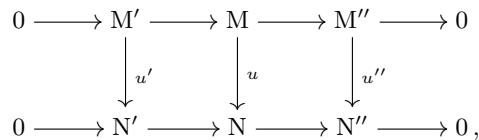
\includegraphics[keepaspectratio]{images/part002_92bb4337.jpg}}

where the first (resp. second) line is an exact sequence of Z{[}G{]}-modules (resp. of Z{[}H{]}-modules) and where \(u', u, u''\) are compatible with \(\varphi\) . Prove that the diagram

\[
\begin{array}{l} \dots \longrightarrow \mathrm{H} ^ {n} (\mathrm{G}, \mathrm{M} ^ {\prime}) \longrightarrow \mathrm{H} ^ {n} (\mathrm{G}, \mathrm{M}) \longrightarrow \mathrm{H} ^ {n} (\mathrm{G}, \mathrm{M} ^ {\prime \prime}) \longrightarrow \mathrm{H} ^ {n + 1} (\mathrm{G}, \mathrm{M} ^ {\prime}) \longrightarrow \dots \\ \Biggl \downarrow_ {\mathrm{H} ^ {n} (\varphi , u ^ {\prime})} \qquad \Biggl \downarrow_ {\mathrm{H} ^ {n} (\varphi , u)} \qquad \Biggl \downarrow_ {\mathrm{H} ^ {n} (\varphi , u ^ {\prime \prime})} \qquad \Biggl \downarrow_ {\mathrm{H} ^ {n + 1} (\varphi , u)} \\ \dots \longrightarrow \mathrm{H} ^ {n} (\mathrm{H}, \mathrm{N} ^ {\prime}) \longrightarrow \mathrm{H} ^ {n} (\mathrm{H}, \mathrm{N}) \longrightarrow \mathrm{H} ^ {n} (\mathrm{H}, \mathrm{N} ^ {\prime \prime}) \longrightarrow \mathrm{H} ^ {n + 1} (\mathrm{H}, \mathrm{N} ^ {\prime}) \longrightarrow \dots \end{array}
\]

(whose horizontal lines are the long exact sequences defined in Exercise 1, c)) is commutative.

\begin{enumerate}
\def\labelenumi{\alph{enumi})}
\setcounter{enumi}{3}
\item
  Examples: If H = G, then the mapping u is compatible with \(Id_{G}\) if and and only if it is Z{[}G{]}-linear, and we have \(\mathrm{H}^{n}(\mathrm{Id}_{\mathrm{G}}, u) = \mathrm{H}^{n}(\mathrm{G}, u)\) . If N is equal to M endowed with the Z{[}G{]}-module structure deduced from \(\varphi\) , then the homomorphisms \(\varphi\) and \(1_{M}\) are compatible; we denote by \(\operatorname{Res}^{q} : \mathrm{H}^{q}(\mathrm{G}, \mathrm{M}) \to \mathrm{H}^{q}(\mathrm{H}, \mathrm{M})\) the homomorphism \(\mathrm{H}^{q}(\varphi, 1_{\mathrm{M}})\) (``restriction homomorphism'').
\item
  Let H be a normal subgroup of G, and let \(M^{H}\) be the subgroup of M consisting of the elements invariant under H, endowed with the action of G/H deduced from that of G by passing to the quotient. The canonical surjection \(p: G \rightarrow G/H\) and the canonical injection \(j: M^{H} \rightarrow M\) are compatible; we denote by \(\operatorname{Inf}^{q}: \operatorname{H}^{q}(\operatorname{G}/\operatorname{H}, \operatorname{M}^{\operatorname{H}}) \to \operatorname{H}^{q}(\operatorname{G}, \operatorname{M})\) the homomorphism \(\operatorname{H}^{q}(p, j)\) (``inflation homomorphism''). Prove that the sequence
\end{enumerate}

\[
0 \to \mathrm{H} ^ {1} (\mathrm{G} / \mathrm{H}, \mathrm{M} ^ {\mathrm{H}}) \xrightarrow {\operatorname{Inf} ^ {1}} \mathrm{H} ^ {1} (\mathrm{G}, \mathrm{M}) \xrightarrow {\operatorname{Res} ^ {1}} \mathrm{H} ^ {1} (\mathrm{H}, \mathrm{M})
\]

is exact. If, moreover, \(\mathrm{H}^1 (\mathrm{H},\mathrm{M})\) is zero, then the sequence

\[
0 \to \mathrm{H} ^ {2} (\mathrm{G} / \mathrm{H}, \mathrm{M} ^ {\mathrm{H}}) \xrightarrow {\operatorname{Inf} ^ {2}} \mathrm{H} ^ {2} (\mathrm{G}, \mathrm{M}) \xrightarrow {\operatorname{Res} ^ {2}} \mathrm{H} ^ {2} (\mathrm{H}, \mathrm{M})
\]

is exact.

¶ 3) Let G be a group and M a Z{[}G{]}-module. Let G act on C \(^{1}\) (G,M) by sending \((g,f)\in\mathrm{G}\times\mathrm{C}^{1}(\mathrm{G},\mathrm{M})\) to the function \(h\mapsto gf(g^{-1}h)\) on G. Recall (I, §6, p.~149, Exercise 8) that a G-mean on M is a Z{[}G{]}-linear mapping \(\mu:C^{1}(\mathrm{G},\mathrm{M})\to\mathrm{M}\) satisfying \(\mu(c_{x})=x\) , where \(c_{x}\) denotes the constant function with value \(x\in\mathrm{M}\) .

\begin{enumerate}
\def\labelenumi{\alph{enumi})}
\item
  Prove that if M admits a G-mean, then \(\mathrm{H}^{n}(\mathrm{G},\mathrm{M})\) is zero for \(n \geqslant 1\) . (For \(q \geqslant 1\) , let \(h^{q}: \mathrm{C}^{q}(\mathrm{G},\mathrm{M}) \to \mathrm{C}^{q-1}(\mathrm{G},\mathrm{M})\) be the following homomorphism: for \(g_{1}, \ldots, g_{q-1}\) in G and \(c \in \mathrm{C}^{q}(\mathrm{G}, \mathrm{M})\) , define \(h^{q}(c)(g_{1}, \ldots, g_{q-1})\) as the image by \(\mu\) of the function \(g \mapsto c(g_{1}, \ldots, g_{q-1}, (g_{1} \cdots g_{q-1})^{-1}g)\) . Prove the equality \(h^{q+1} \circ d^{q} + d^{q-1} \circ h^{q} = 1_{\mathrm{C}^{q}(\mathrm{G}, \mathrm{M})}\) .
\item
  Let A be an abelian group; denote by \(\mathcal{F}(\mathrm{G},\mathrm{A})\) the group of mappings from G to A, endowed with the action of G defined by \({}^{g}f(h)=f(hg)\) for g,h in G and f in \(\mathcal{F}(\mathrm{G},\mathrm{A})\) . For any mapping c from G to \(\mathcal{F}(\mathrm{G},\mathrm{A})\) , denote by \(\mu(c)\) the mapping \(g\mapsto c(g^{-1})(g)\) from G to A. Show that \(\mu\) is a G-mean on \(\mathcal{F}(\mathrm{G},\mathrm{A})\) ; we therefore have \(\mathrm{H}^{q}(\mathrm{G},\mathcal{F}(\mathrm{G},\mathrm{A}))=0\) for \(q\geqslant1\) .
\item
  Let \(j: M \to \mathcal{F}(G, M)\) be the mapping that sends an element m of M to the function \(g \mapsto gm\) , and let \(M'\) be its cokernel. Prove that j is injective and Z{[}G{]}-linear. Deduce that the homomorphism \(\partial^{q}: H^{q}(G, M') \to H^{q+1}(G, M)\) is bijective for \(q \geqslant 1\) .
\item
  Let L be a finite Galois extension of the commutative field K and G be its Galois group. Deduce from b) and the normal basis theorem (V, §10, No.~9, p.~73) that the groups \(\mathrm{H}^{n}(\mathrm{G},\mathrm{L})\) are zero for \(n \geqslant 1\) .
\end{enumerate}

¶ 4) Let G be a group and H a subgroup of G. For any Z{[}H{]}-module N, denote by \(\widetilde{N}\) the group \(\operatorname{Hom}_{\mathbf{Z}[H]}(\mathbf{Z}[G], N)\) endowed with a Z{[}G{]}-module structure deduced from the right Z{[}G{]}-module structure on Z{[}G{]}.

\begin{enumerate}
\def\labelenumi{\alph{enumi})}
\item
  Prove that \(\widetilde{\mathbf{N}}\) can be identified with the \(\mathbf{Z}[\mathrm{G}]\) -submodule of \(\mathcal{F}(\mathrm{G},\mathrm{N})\) (Exercise 3) consisting of the mappings \(f\) such that \(f(hg) = hf(g)\) for every \(h\in \mathrm{H}\) and \(g\in \mathrm{G}\) . If \(\mathrm{A}\) is an abelian group, then the \(\mathbf{Z}[\mathrm{G}]\) -module \(\widetilde{\mathcal{F}(\mathrm{H},\mathrm{A})}\) is canonically isomorphic to \(\mathcal{F}(\mathrm{G},\mathrm{A})\) .
\item
  Let \(0 \rightarrow N' \stackrel{i}{\rightarrow} N \stackrel{p}{\rightarrow} N'' \rightarrow 0\) be an exact sequence of Z{[}H{]}-modules; the sequence
\end{enumerate}

\[
0 \longrightarrow \widetilde {\mathrm{N}} ^ {\prime} \xrightarrow {\operatorname{Hom} (1 , i)} \widetilde {\mathrm{N}} \xrightarrow {\operatorname{Hom} (1 , p)} \widetilde {\mathrm{N}} ^ {\prime \prime} \longrightarrow 0
\]

is exact (observe that the \(\mathbf{Z}[\mathrm{H}]\) -module \(\mathbf{Z}[\mathrm{G}]\) is free).

\begin{enumerate}
\def\labelenumi{\alph{enumi})}
\setcounter{enumi}{2}
\tightlist
\item
  Let \(u_{N} : \widetilde{N} \to N\) be the mapping \(f \mapsto f(1)\) ; it is compatible with the canonical injection \(i : H \to G\) (Exercise 2). Prove that the homomorphism
\end{enumerate}

\[
\mathrm{H} ^ {q} (i, u _ {\mathrm{N}}): \mathrm{H} ^ {q} (\mathrm{G}, \widetilde {\mathrm{N}}) \to \mathrm{H} ^ {q} (\mathrm{H}, \mathrm{N})
\]

is bijective for every \(q \geqslant 0\) (first treat the case q = 0 and then reason by induction on q using the above; Exercise 3, c); and Exercise 2, c)).

\begin{enumerate}
\def\labelenumi{\alph{enumi})}
\setcounter{enumi}{3}
\item
  Suppose that H has finite index n in G. Let M be a Z{[}G{]}-module, which we view as a Z{[}H{]}-module by restriction of scalars. Let \(f \in \widetilde{M}\) ; the element \(g^{-1}f(g)\) depends only on the right class Hg of g. Set \(\pi(f) = \sum_{Hg \in H \setminus G} g^{-1}f(g)\) . Prove that \(\pi\) is a Z{[}G{]}-linear homomorphism from \(\widetilde{M}\) to M. For any integer \(q \geqslant 0\) , denote by \(\operatorname{Cor}^{q}: \mathrm{H}^{q}(\mathrm{H}, \mathrm{M}) \to \mathrm{H}^{q}(\mathrm{G}, \mathrm{M})\) the homomorphism \(\mathrm{H}^{q}(\pi) \circ \mathrm{H}^{q}(i, u_{\mathrm{M}})^{-1}\) (``corestriction homomorphism'').
\item
  Prove that the endomorphism \(Cor^{q} \circ Res^{q}\) of \(H^{q}(G, M)\) is multiplication by n (first treat the case q = 0 and then treat the general case as in the proof of c)).
\item
  Suppose that G is finite; prove that for every Z{[}G{]}-module M and every integer \(q \geqslant 1\) , the group \(\mathrm{H}^{q}(\mathrm{G}, \mathrm{M})\) is annihilated by the order of G.
\end{enumerate}

\begin{enumerate}
\def\labelenumi{\arabic{enumi})}
\setcounter{enumi}{4}
\tightlist
\item
  Let G be a group and M a not necessarily abelian group endowed with a homomorphism \(\varphi: G \to \text{Aut}(M)\) ; for \(g \in G\) and \(m \in M\) , set \(^{g}m = \varphi(g)(m)\) . Denote by \(H^{0}(G, M)\) the subgroup of M consisting of the elements fixed by the action of G; its identity element is called the marked or distinguished element of \(H^{0}(G, M)\) . Let \(Z^{1}(G, M)\) be the set of mappings \(c: G \to M\) satisfying \(c(gh) = c(g)^{g}c(h)\) for g, h in G. For \(c \in Z^{1}(G, M)\) and \(m \in M\) , the mapping \(g \mapsto mc(g)(^g m)^{-1}\) belongs to \(Z^{1}(G, M)\) ; this defines an action of the group M on \(Z^{1}(G, M)\) . The quotient set is denoted by \(H^{1}(G, M)\) ; it is endowed with a marked element, namely the class of the constant mapping with value 1. If M is abelian, then the set \(H^{1}(G, M)\) coincides with that defined in Exercise 1.
\end{enumerate}

\begin{enumerate}
\def\labelenumi{\alph{enumi})}
\item
  Let N be a second group endowed with an action of G and \(u: M \to N\) a group homomorphism compatible with the actions of G. For i = 0, 1, define homomorphisms \(\mathrm{H}^{i}(u): \mathrm{H}^{i}(\mathrm{G}, \mathrm{M}) \to \mathrm{H}^{i}(\mathrm{G}, \mathrm{N})\) that send the marked element of \(\mathrm{H}^{i}(\mathrm{G}, \mathrm{M})\) to that of \(\mathrm{H}^{i}(\mathrm{G}, \mathrm{N})\) .
\item
  Let \(0 \to M' \xrightarrow{\iota} M \xrightarrow{\pi} M'' \to 0\) be an exact sequence of groups with operators in G. Let \(x'' \in \mathrm{H}^0(\mathrm{G}, \mathrm{M}'')\) , and let x be an element of M such that \(\pi(x) = x''\) . Prove that there exists an element \(c' \in \mathrm{Z}^1(\mathrm{G}, \mathrm{M}')\) such that \(\iota \circ c'(g) = g^{-1}c(g)\) for every \(g \in G\) and that the class of \(c'\) in \(\mathrm{H}^1(\mathrm{G}, \mathrm{M}')\) depends only on \(x''\) ; we denote that class by \(\partial(x'')\) . Prove that the sequence
\end{enumerate}

\[
0 \to \mathrm{H} ^ {0} (\mathrm{G}, \mathrm{M} ^ {\prime}) \xrightarrow {\mathrm{H} ^ {0} (\iota)} \mathrm{H} ^ {0} (\mathrm{G}, \mathrm{M}) \xrightarrow {\mathrm{H} ^ {0} (\pi)} \mathrm{H} ^ {0} (\mathrm{G}, \mathrm{M} ^ {\prime \prime}) \xrightarrow {\partial}
\]

\[
\mathrm{H} ^ {1} (\mathrm{G}, \mathrm{M} ^ {\prime}) \xrightarrow {\mathrm{H} ^ {1} (\iota)} \mathrm{H} ^ {1} (\mathrm{G}, \mathrm{M}) \xrightarrow {\mathrm{H} ^ {1} (\pi)} \mathrm{H} ^ {1} (\mathrm{G}, \mathrm{M} ^ {\prime \prime})
\]

is exact (a sequence of mappings \(G \xrightarrow{i} F \xrightarrow{p} E\) , where the set E is endowed with a marked element e, is called exact in F if \(\operatorname{Im}(i) = p^{-1}(e)\) ).

\begin{enumerate}
\def\labelenumi{\alph{enumi})}
\setcounter{enumi}{2}
\item
  Suppose, moreover, that \(M'\) is contained in the center of M. Construct a mapping \(\partial^{1}: H^{1}(G, M'') \to H^{2}(G, M')\) such that the inverse image of the identity element by \(\partial^{1}\) is the image of \(H^{1}(\pi)\) . Also define an action of the group \(H^{1}(G, M')\) on the set \(H^{1}(G, M)\) such that two elements are conjugate for this action if and only if they have the same image by \(H^{1}(\pi)\) .
\item
  Let K be a commutative field, L a finite Galois extension of K with Galois group G, and n an integer. Let G act on the group \(\mathbf{GL}_{n}(\mathrm{L})\) by setting \(\sigma A = (\sigma(a_{ij}))\) for \(\sigma \in G\) and \(A = (a_{ij}) \in \mathbf{GL}_{n}(\mathrm{L})\) . Deduce from V, §10, No.~5, p.~64, Proposition 9 that the set \(\mathrm{H}^{1}(\mathrm{G}, \mathbf{GL}_{n}(\mathrm{L}))\) is reduced to one element (``Hilbert's 90 theorem'').
\end{enumerate}

¶ 6) Let L be a finite Galois extension of the commutative field K, with Galois group G. Let V and V' be K-vector spaces and w (resp. w') a tensor of type \((p,q)\) on V (resp. V'). An L-isomorphism from \((V,w)\) to \((V',w')\) is an L-linear isomorphism \(u:V_{(L)}\to V_{(L)}'\) such that \(u^{\otimes p}\otimes(^{t}u^{-1})^{\otimes q}\) sends the image of w to that of \(w'\) . We denote by \(\operatorname{Aut}_{\mathrm{L}}(\mathrm{V},w)\) the group of L-automorphisms of \((\mathrm{V},w)\) , on which G acts by \(\sigma\varphi=(1_{\mathrm{V}}\otimes\sigma)\circ\varphi\circ(1_{\mathrm{V}}\otimes\sigma)^{-1}\) .

\begin{enumerate}
\def\labelenumi{\alph{enumi})}
\item
  Let u be an L-isomorphism from \((\mathrm{V}, w)\) to \((\mathrm{V}^{\prime}, w^{\prime})\) and \(\sigma\) an element of G; the mapping \(\sigma u = (1_{\mathrm{V}^{\prime}} \otimes \sigma) \circ u \circ (1_{\mathrm{V}} \otimes \sigma)^{-1}\) is an L-isomorphism from \((\mathrm{V}, w)\) to \((\mathrm{V}^{\prime}, w^{\prime})\) , so that \(c(\sigma) = u^{-1} \circ \sigma u\) is an element of \(\operatorname{Aut}_{\mathrm{L}}(\mathrm{V}, w)\) . Prove that the mapping \(c : G \to \operatorname{Aut}_{\mathrm{L}}(\mathrm{V}, w)\) belongs to \(Z^{1}(\mathrm{G}, \operatorname{Aut}_{\mathrm{L}}(\mathrm{V}, w))\) and that its class \(\theta(\mathrm{V}^{\prime}, w^{\prime})\) in \(H^{1}(\mathrm{G}, \operatorname{Aut}_{\mathrm{L}}(\mathrm{V}, w))\) does not depend on the choice of u.
\item
  Prove that the mapping \((\mathrm{V}^{\prime},t^{\prime})\mapsto\theta(\mathrm{V}^{\prime},t^{\prime})\) defines a bijection from the set of K-isomorphism classes of pairs \((\mathrm{V}^{\prime},w^{\prime})\) L-isomorphic to \((\mathrm{V},w)\) to the set \(\mathrm{H}^{1}(\mathrm{G},\mathrm{Aut}_{\mathrm{L}}(\mathrm{V},w))\) . (Given an element c of \(\mathrm{Z}^{1}(\mathrm{G},\mathrm{Aut}_{\mathrm{L}}(\mathrm{V},w))\) , deduce from Exercise 5, d) an L-automorphism f of \(\mathrm{V}_{(\mathrm{L})}\) such that \(c(\sigma)=f^{-1}\circ^{\sigma}f\) . Prove that the image \(w^{\prime}\) of w by the automorphism deduced from f is rational over K, and consider the pair \((\mathrm{V},w^{\prime}).\) )
\end{enumerate}

* c) Examples: The set \(\mathrm{H}^1 (\mathrm{G},\mathbf{Sp}_{2n}(\mathrm{L}))\) is reduced to one element. If Q is a quadratic form on K, then the set \(\mathrm{H}^1 (\mathrm{G},\mathbf{O}(\mathrm{Q}_{(\mathrm{L})}))\) can be identified with the set of equivalence classes of quadratic forms on K equivalent to Q over L.*

\(d\) ) Let A be a K-algebra and M the automorphism group of the L-algebra \(\mathrm{A}_{(\mathrm{L})}\) , endowed with the action of G defined above. The construction in \(b\) ) defines a bijection from the set of isomorphism classes of pairs \((\mathrm{B},u)\) , where B is a K-algebra and \(u\) is an isomorphism from \(\mathrm{B}_{(\mathrm{L})}\) to \(\mathrm{A}_{(\mathrm{L})}\) , to the set \(Z^{1}(\mathrm{G},\mathrm{M})\) . The inverse bijection sends an element \(c\) of \(Z^{1}(\mathrm{G},\mathrm{M})\) to the K-subalgebra of \(\mathrm{A}_{(\mathrm{L})}\) consisting of the elements \(a\) satisfying \(c(\sigma)(\sigma(a)) = a\) for every \(\sigma \in \mathrm{G}\) .

\begin{enumerate}
\def\labelenumi{\arabic{enumi})}
\setcounter{enumi}{6}
\tightlist
\item
  Let L be an extension of K. For any integer \(n \geqslant 1\) , denote by \(\mathcal{A}_{n}(\mathrm{L}/\mathrm{K})\) the set of isomorphism classes of central simple K-algebras of degree \(n^{2}\) split by L.
\end{enumerate}

\begin{enumerate}
\def\labelenumi{\alph{enumi})}
\item
  Prove that the kernel \(\mathrm{Br}(\mathrm{L} / \mathrm{K})\) of the canonical homomorphism \(\mathrm{Br}(\mathrm{K})\to \mathrm{Br}(\mathrm{L})\) is isomorphic to the direct limit of the sets \(\mathcal{A}_n(\mathrm{L} / \mathrm{K})\) ; specify a system of mappings. b) Assume from now on that L is a finite Galois extension of K, with Galois group G. Deduce a bijection \(\theta_{n}:\mathcal{A}_{n}(\mathrm{L} / \mathrm{K})\to \mathrm{H}^{1}(\mathrm{G},\mathbf{PGL}_{n}(\mathrm{L}))\) from Exercise 6.
\item
  Denote by \(\partial_n: \mathrm{H}^1(\mathrm{G}, \mathbf{PGL}_n(\mathrm{L})) \to \mathrm{H}^2(\mathrm{G}, \mathrm{L}^*)\) the mapping deduced from the exact sequence \(1 \to \mathrm{L}^* \to \mathbf{GL}_n(\mathrm{L}) \to \mathbf{PGL}_n(\mathrm{L}) \to 1\) (Exercise 5, c)) and by \(\delta_n: \mathcal{A}_n(\mathrm{L/K}) \to \mathrm{H}^2(\mathrm{G}, \mathrm{L}^*)\) the mapping \(\partial_n \circ \theta_n\) . If \(\mathrm{A} \in \mathcal{A}_n(\mathrm{L/K})\) , then we have \(\delta_n(\mathrm{A}) = 0\) if and only if \(\mathrm{A}\) is a matrix algebra over \(\mathrm{K}\) ; if \(\mathrm{A} \in \mathcal{A}_p(\mathrm{L/K})\) and \(\mathrm{B} \in \mathcal{A}_q(\mathrm{L/K})\) , then we have \(\delta_{pq}(\mathrm{A} \otimes_{\mathrm{K}} \mathrm{B}) = \delta_p(\mathrm{A}) + \delta_q(\mathrm{B})\) . Deduce an injective group homomorphism \(\delta_{\mathrm{L/K}}: \mathrm{Br}(\mathrm{L/K}) \to \mathrm{H}^2(\mathrm{G}, \mathrm{L}^*)\) by passing to the direct limit. d) Prove that \(\partial_n\) is surjective for \(n = \operatorname{Card}(\mathrm{G})\) . (Let \(c: \mathrm{G} \times \mathrm{G} \to \mathrm{L}^*\) be an element of \(\mathrm{Z}^2(\mathrm{G}, \mathrm{L}^*)\) . For every \(\sigma \in \mathrm{G}\) , consider the endomorphism \(u(\sigma)\) of \(\mathrm{L}^{\mathrm{G}}\) that sends \(e_\tau\) to \(c(\sigma, \tau)e_{\sigma\tau}\) for every \(\tau \in \mathrm{G}\) , and determine \(u(\sigma)^{\sigma}u(\tau)u(\sigma\tau)^{-1}\) .)
\item
  Compare \(\delta_{\mathrm{L / K}}\) and \(\Phi_{\mathrm{L / K}}\) .
\item
  Prove that the group \(\mathrm{Br}(\mathrm{K})\) can be identified with the limit of the direct system of groups \(\left(\mathrm{H}^{2}(\mathrm{Gal}(\mathrm{L}/\mathrm{K}),\mathrm{L}^{*})\right)\) with respect to the set (ordered by inclusion) of finite Galois extensions of K contained in a fixed algebraic closure of K, where the homomorphisms between these groups are the (injective) inflation homomorphisms. g) Let F be an extension of K contained in L and \(\Gamma\) the subgroup of G that leaves F invariant. Prove that the following diagram commutes:
\end{enumerate}

\[
\begin{array}{c} \operatorname{Br} (\mathrm{L} / \mathrm{K}) \xrightarrow {r _ {\mathrm{F} / \mathrm{K}}} \operatorname{Br} (\mathrm{F} / \mathrm{L}) \\ \Biggl \downarrow_ {\delta_ {\mathrm{L} / \mathrm{K}}} \qquad \qquad \qquad \qquad \Biggl \downarrow_ {\delta_ {\mathrm{F} / \mathrm{L}}} \\ \operatorname{H} ^ {2} (\operatorname{G}, \operatorname{L} ^ {*}) \xrightarrow {\operatorname{Res} ^ {2}} \operatorname{H} ^ {2} (\Gamma , \operatorname{L} ^ {*}). \end{array}
\]

Deduce a canonical isomorphism from \(\mathrm{Br}(\mathrm{F}/\mathrm{K})\) to the kernel of the homomorphism \(\mathrm{Res}^{2}:\mathrm{H}^{2}(\mathrm{G},\mathrm{L}^{*})\to\mathrm{H}^{2}(\Gamma,\mathrm{L}^{*})\) .

\begin{enumerate}
\def\labelenumi{\arabic{enumi})}
\setcounter{enumi}{7}
\item
  Let L be an extension of K. Suppose that K has characteristic p \textgreater{} 0 and \(L = K^{1/p}\) . Prove that the group \(\mathrm{Br}(\mathrm{L}/\mathrm{K})\) is equal to the kernel of multiplication by p in \(\mathrm{Br}(\mathrm{K})\) (observe that if N is a finite Galois extension of K, then \(N^{1/p}\) is a Galois extension of L with the same Galois group).
\item
  Let G be a finite group and M a Z{[}G{]}-module. Denote by \(N_{G}\) the homomorphism \(m \mapsto \sum_{g} gm\) from M to M; its image is contained in the submodule \(M^{G}\) of M consisting of the invariant elements. Let \(\mathrm{T}_{\mathrm{G}}(\mathrm{M})\) be the quotient group \(\mathrm{M}^{\mathrm{G}}/\mathrm{N}_{\mathrm{G}}(\mathrm{M})\) . a) Let \(c \in \mathrm{Z}^{2}(\mathrm{G}, \mathrm{M})\) . Prove that the element \(\sum_{h} c(h, g)\) belongs to \(M^{G}\) ; we denote its class in \(\mathrm{T}_{\mathrm{G}}(\mathrm{M})\) by \(\theta_{c}(g)\) . Prove that \(\theta_{c}\) is a homomorphism from G to \(\mathrm{T}_{\mathrm{G}}(\mathrm{M})\) that is zero when \(c \in \mathrm{B}^{2}(\mathrm{G}, \mathrm{M})\) . Deduce a homomorphism \(\theta_{\mathrm{M}} : \mathrm{H}^{2}(\mathrm{G}, \mathrm{M}) \to \mathrm{Hom}(\mathrm{G}, \mathrm{T}_{\mathrm{G}}(\mathrm{M}))\) from it.
\end{enumerate}

\begin{enumerate}
\def\labelenumi{\alph{enumi})}
\setcounter{enumi}{1}
\tightlist
\item
  Let \(u: M \to N\) be a homomorphism of Z{[}G{]}-modules and \(\widetilde{u}: T_{G}(M) \to T_{G}(N)\) the homomorphism induced by u. Prove that we have \(\theta_{\mathrm{N}} \circ \mathrm{H}^{2}(u) = \mathrm{Hom}(1_{\mathrm{G}}, \widetilde{u}) \circ \theta_{\mathrm{M}}\) . c) Assume from now on that G is cyclic; let \(\sigma\) be a generator of G, and denote its order by n.~Let \(\chi \in \mathrm{Hom}(G, \mathbf{Z}/n\mathbf{Z})\) be the homomorphism that sends \(\sigma\) to the class of 1, and let \(\lambda \in H^{2}(G, \mathbf{Z})\) be its image by the connecting homomorphism associated with the exact sequence \(0 \to Z \to Z \to Z/nZ \to 0\) . Prove that \(\lambda\) is the class of the element \(\varepsilon \in Z^{2}(G, \mathbf{Z})\) such that for \(0 \leqslant p < n\) and \(0 \leqslant q < n\) , the image \(\varepsilon(\sigma^{p}, \sigma^{q})\) is equal to 0 if \(p + q < n\) and to 1 if \(p + q \geqslant n\) . For \(m \in M^{G}\) , denote by \(h_{m}\) the Z{[}G{]}-linear mapping from Z to M such that \(h_{m}(1) = m\) . Prove that the image of \(H^{2}(h_{m})(\lambda)\) by \(\theta_{M}\) is equal to the class of m, so that \(\theta_{M}\) is surjective.
\end{enumerate}

\(d\) ) Prove that \(\theta_{\mathrm{M}}\) is an isomorphism. (Let \(c\in \mathbf{Z}^2 (\mathrm{G},\mathrm{M})\) . Prove that we may assume \(c(g,1) = c(1,g) = 1\) for every \(g\in \mathrm{G}\) , and determine the images by \(d^1\) of the elements \(b\) and \(a_{m}\) \((m\in \mathrm{M})\) of \(\mathrm{C}^1 (\mathrm{G},\mathrm{M})\) defined by \(b(\sigma^{p}) = \sum_{i = 0}^{p - 1}c(\sigma^{i},\sigma)\) and \(a_{m}(\sigma^{p}) = \sum_{i = 0}^{p - 1}\sigma^{i}m.)\)

\begin{enumerate}
\def\labelenumi{\arabic{enumi})}
\setcounter{enumi}{9}
\tightlist
\item
  \begin{enumerate}
  \def\labelenumii{\alph{enumii})}
  \tightlist
  \item
    Let L be a cyclic extension of K. Deduce from Exercises 9 and 7 that the groups Br(L/K) and \(K^{*}/N_{L/K}(L^{*})\) are isomorphic.
  \end{enumerate}
\end{enumerate}

\begin{enumerate}
\def\labelenumi{\alph{enumi})}
\setcounter{enumi}{1}
\item
  Suppose that every extension L of K of finite degree is cyclic and that the norm mapping \(N_{L/K}: L^{*} \to K^{*}\) is surjective. Prove that every field extension of K of finite degree with center K is equal to K.
\item
  Apply the previous question to finite fields.
\end{enumerate}

\begin{enumerate}
\def\labelenumi{\arabic{enumi})}
\setcounter{enumi}{10}
\tightlist
\item
  Let L be a cyclic extension of K with Galois group G, and let \(\sigma\) be a generator of G. Exercise 10 gives a canonical isomorphism \(\mathrm{Br}(\mathrm{L}/\mathrm{K}) \to \mathrm{K}^{*}/\mathrm{N}_{\mathrm{L}/\mathrm{K}}(\mathrm{L}^{*})\) , whose inverse we will now construct explicitly.
\end{enumerate}

Let \(\theta \in \mathrm{K}^*\) , and let \(c_{\theta} \in \mathrm{Z}^{2}(\mathrm{G}, \mathrm{L}^{*})\) be the element defined by \(c_{\theta}(\sigma^{p}, \sigma^{q}) = \theta^{\varepsilon(p,q)}\) (Exercise 9, \(c\) )). Prove that the cross product A{[} \(\mathcal{E}\) , L{]} of L and the extension \(\mathcal{E}\) associated with \(c_{\theta}\) is isomorphic to the quotient of the K-algebra L{[}X{]} \(_{\sigma}\) (VIII, p.~11) by the (two-sided) ideal generated by the central element X \(^{n}\) - \(\theta\) . The class of A \(_{\theta}\) in Br(L/K) corresponds to the class of \(\theta\) ( \(\text{mod } \mathrm{N}_{\mathrm{L/K}}(\mathrm{L}^{*})\) ) by the isomorphism defined above.

\begin{enumerate}
\def\labelenumi{\arabic{enumi})}
\setcounter{enumi}{11}
\tightlist
\item
  Let A be a commutative ring. Endow the set of isomorphism classes of Azumaya A-algebras (VIII, p.~270, Exercise 8) with the structure of a monoid by setting \(\operatorname{cl}(S)\operatorname{cl}(T)=\operatorname{cl}(S\otimes_{A}T)\) .
\end{enumerate}

\begin{enumerate}
\def\labelenumi{\alph{enumi})}
\item
  Prove that the quotient monoid for Morita equivalence is an abelian group; we denote it by Br(A) and call it the Brauer group of A (when A is a field, this definition coincides with that given in VIII, p.~279). Denote by {[}S{]} the class of an Azumaya A-algebra S in Br(A). The identity element of Br(A) is the class of A, and the inverse of an element {[}S{]} is {[}S°{]}.
\item
  Let S be an Azumaya A-algebra. We have \([S] = [A]\) if and only if there exists a finitely generated, projective, faithful A-module P such that S is isomorphic to \(\operatorname{End}_{\mathrm{A}}(\mathrm{P})\) .
\item
  Let B be a commutative A-algebra. Define a group homomorphism \(r_{B/A} : \mathrm{Br}(A) \to \mathrm{Br}(B)\) such that \(r_{\mathrm{B/A}}([\mathrm{S}]) = [\mathrm{S}_{(\mathrm{B})}]\) for every Azumaya A-algebra S. We denote the kernel of this homomorphism by \(\mathrm{Br(B/A)}\) .
\end{enumerate}

¶ 13) Let A be a commutative ring, B a commutative A-algebra, and G a finite group of automorphisms of the A-algebra B. Suppose that B is a finitely generated, projective, faithful A-module and that the A-linear homomorphism \(\psi : \mathrm{B} \otimes_{\mathrm{A}} \mathrm{B} \to \mathrm{B}^{\mathrm{G}}\) defined by \(\psi(b \otimes b') = (\sigma(b)b')_{\sigma \in \mathrm{G}}\) is bijective.

\begin{enumerate}
\def\labelenumi{\alph{enumi})}
\item
  Let N be a B-module, endowed with a homomorphism \(\sigma \mapsto u_{\sigma}\) from G to \(\mathrm{Aut}_{\mathrm{A}}(\mathrm{N})\) satisfying \(u_{\sigma}(bx) = \sigma(b)u_{\sigma}(x)\) for \(\sigma \in \mathrm{G}\) , \(b \in \mathrm{B}\) , \(x \in \mathrm{N}\) . Let M be the A-submodule of N consisting of the elements \(x\) such that \(u_{\sigma}(x) = x\) for every \(\sigma \in \mathrm{G}\) . Prove that the canonical B-homomorphism \(\mathrm{B} \otimes_{\mathrm{A}} \mathrm{M} \to \mathrm{N}\) is bijective (use Exercise 7, \(d\) ) of VIII, p.~270 to reduce to the case when B is the product algebra \(\mathrm{A}^{\mathrm{G}}\) on which G acts by permuting the factors).
\item
  Let S be an A-algebra and M the automorphism group of the B-algebra \(\mathrm{S}_{(\mathrm{B})}\) , on which G acts by \(\sigma\varphi = (\mathrm{Id}_{\mathrm{S}} \otimes \sigma) \circ \varphi \circ (\mathrm{Id}_{\mathrm{S}} \otimes \sigma)^{-1}\) . Extend the construction of Exercise 6 to define a bijection from the set of isomorphism classes of pairs \((T,u)\) , where T is an A-algebra and u an isomorphism from \(T_{(B)}\) to \(S_{(B)}\) , to the set \(Z^{1}(G,M)\) , as well as a bijection from the set of isomorphism classes of A-algebras T such that the B-algebras \(T_{(B)}\) and \(S_{(B)}\) are isomorphic to \(H^{1}(G,M)\) .
\item
  Assume from now on that every projective B-module is free. Adapt the reasoning of Exercise 8 to construct an isomorphism \(\theta : \mathrm{Br}(\mathrm{B} / \mathrm{A}) \to \mathrm{H}^2(\mathrm{G}, \mathrm{B}^*)\) .
\end{enumerate}

¶ 14) Let A be a Noetherian commutative local ring, m its maximal ideal, \(\kappa\) the field A/m, and S an Azumaya algebra over A.

\begin{enumerate}
\def\labelenumi{\alph{enumi})}
\item
  Let \(e\) be an idempotent in S whose image in S/mS is an indecomposable idempotent. Deduce from Nakayama's lemma (cf.~VIII, p.~168, Exercise 16) that the canonical homomorphism \(S \to \mathrm{End}_{\mathrm{A}}(Se)\) is bijective.
\item
  Suppose that m is nilpotent \(^{*}\) (or, more generally, that A is complete for the m-adic topology) \(^{*}\) . Prove that the homomorphism \(r_{\kappa/A}: \mathrm{Br}(A) \to \mathrm{Br}(\kappa)\) is injective.
\end{enumerate}

* \(c\) ) Assume from now on that A is complete. Let L be a separable extension of \(\kappa\) of finite degree that is a splitting field for the \(\kappa\) -algebra S/mS. Let \(x\) be a primitive element of L, \(f\) its minimal polynomial, F a monic polynomial in A{[}X{]} whose image in \(\kappa\) {[}X{]} is \(f\) , and B = A{[}X{]}/(F). Prove that B is a local A-algebra, free and finitely generated as an A-module, with maximal ideal mB and residue field isomorphic to L; the B-algebra S \(_{(B)}\) is isomorphic to a matrix algebra.

\(d\) ) Suppose, moreover, that L is a Galois extension of \(\kappa\) , with Galois group G. Prove that the action of G on L lifts to an action on the A-algebra B (let \(G'\) be the automorphism group of this algebra; deduce from Hensel's lemma (Comm. Alg., III, §4, No.~3, p.~215, Theorem 1) that the natural homomorphism \(G' \to G\) is bijective). Deduce from Nakayama's lemma that the homomorphism \(\psi : B \otimes_A B \to B^G\) defined in Exercise 13 is bijective.

\begin{enumerate}
\def\labelenumi{\alph{enumi})}
\setcounter{enumi}{4}
\item
  Prove that the homomorphism \(\mathrm{H}^{q}(\pi):\mathrm{H}^{q}(\mathrm{G},\mathrm{B}^{*})\to\mathrm{H}^{q}(\mathrm{G},\mathrm{L}^{*})\) is bijective for every \(q\geqslant1\) . (For \(i\geqslant1\) , let \(U^{i}\) be the subgroup of elements b of \(B^{*}\) such that \(b\equiv1\) (mod \(m^{i}B\) ). Observe that the Z{[}G{]}-module \(U^{i}/U^{i+1}\) is isomorphic to \(m^{i}B/m^{i+1}B\) , hence to a power of L, and deduce from Exercise 5, d) that \(\mathrm{H}^{q}(\mathrm{G},\mathrm{U}^{i}/\mathrm{U}^{i+1})\) is zero for \(q\geqslant1\) . Let \(c\in\mathrm{Z}^{q}(\mathrm{G},\mathrm{U}^{1})\) . Construct, by induction, a sequence \((b_{n})\) with \(b_{n}\in\mathrm{Z}^{q-1}(\mathrm{G},\mathrm{U}^{n})\) such that \(c-d^{q-1}(\sum_{i=1}^{n}b_{i})\) belongs to \(\mathrm{Z}^{q}(\mathrm{G},\mathrm{U}^{n+1})\) . Conclude that \(\mathrm{H}^{q}(\mathrm{G},\mathrm{U}^{1})\) is zero for \(q\geqslant1\) .
\item
  Conclude that the canonical homomorphisms \(\mathrm{Br}(B/A)\to \mathrm{Br}(L/\kappa)\) and \(\mathrm{Br}(A)\to \mathrm{Br}(\kappa)\) are bijective.*
\end{enumerate}

\begin{enumerate}
\def\labelenumi{\arabic{enumi})}
\setcounter{enumi}{14}
\tightlist
\item
  *a) Let A be a regular integral domain (AC, X, §4, n° 2, p.~55) and K its field of fractions. The homomorphism \(r_{\mathrm{K / A}}: \mathrm{Br(A)} \to \mathrm{Br(K)}\) is injective (VIII, p.~271, Exercise 11).*
\end{enumerate}

\begin{enumerate}
\def\labelenumi{\alph{enumi})}
\setcounter{enumi}{1}
\tightlist
\item
  Prove that the ring \(A = \mathbf{Q}[X, Y]/(X^{2} + Y^{2})\) is an integral domain; let K be its field of fractions. Let H be the quaternion algebra of type \((-1, 0, -1)\) over Q, which is a field (cf.~III, §2, No.~5, p.~445). Prove that the class of the Azumaya
\end{enumerate}

A-algebra \(\mathrm{H}_{(\mathrm{A})}\) in \(\mathrm{Br}(\mathrm{A})\) is not zero but that \(\mathrm{H}_{(\mathrm{K})}\) is isomorphic to \(\mathbf{M}_{2}(\mathrm{K})\) , so that the homomorphism \(r_{K/A}\) is not injective (observe that K contains an element of square -1).

\begin{enumerate}
\def\labelenumi{\arabic{enumi})}
\setcounter{enumi}{15}
\tightlist
\item
  \begin{enumerate}
  \def\labelenumii{\alph{enumii})}
  \tightlist
  \item
    Prove that the homomorphism \(r_{\mathrm{K[X]}/\mathrm{K}} : \mathrm{Br}(\mathrm{K}) \to \mathrm{Br}(\mathrm{K}[\mathrm{X}])\) induces an isomorphism from \(\mathrm{Br}(\mathrm{K})\) to a direct factor of \(\mathrm{Br}(\mathrm{K}[\mathrm{X}])\) .
  \end{enumerate}
\end{enumerate}

\(^{*}b\) ) Suppose that the field K is perfect. Prove that \(r_{K[X]/K}\) is an isomorphism (deduce from Tsen's theorem (VIII, p.~360, Exercise 7) that \(\mathrm{Br}(\mathrm{K}[\mathrm{X}])\) is the union of the groups \(\mathrm{Br}(\mathrm{L}[\mathrm{X}]/\mathrm{K}[\mathrm{X}])\) , where L runs through the Galois extensions of K of finite degree, and then apply Exercise 13).

\begin{enumerate}
\def\labelenumi{\alph{enumi})}
\setcounter{enumi}{2}
\tightlist
\item
  Let A be a regular Q-algebra that is an integral domain. Prove that the homomorphism \(r_{\mathrm{A[X]}/\mathrm{A}} : \mathrm{Br}(\mathrm{A}) \to \mathrm{Br}(\mathrm{A}[\mathrm{X}])\) is bijective (use b) and Exercise 15 to prove that the homomorphism \(\mathrm{Br}(\mathrm{A}[\mathrm{X}]) \to \mathrm{Br}(\mathrm{A})\) deduced from the surjection \(\mathrm{P} \mapsto \mathrm{P}(0)\) is injective).*
\end{enumerate}

\(d\) ) Suppose that K has characteristic \(p > 0\) and is not perfect; let \(\theta \in \mathrm{K} - \mathrm{K}^p\) . View \(\mathrm{B} = \mathrm{K}[\mathrm{U}]\) as a K{[}X{]}-algebra via the homomorphism \(\rho : \mathrm{K}[\mathrm{X}] \to \mathrm{B}\) determined by \(\rho (\mathrm{X}) = \mathrm{U}^p - \mathrm{U}\) . Let \(\sigma\) be the automorphism of this K{[}X{]}-algebra such that \(\sigma (\mathrm{U}) = \mathrm{U} + 1\) , and let S be the quotient K{[}X{]}-algebra of B{[}V{]}\(_{\sigma}\) (VIII, p.~11) by the two-sided ideal B(\(V^{p} - \theta\)). Let L be a K{[}X{]}-algebra that is a commutative field. Prove that if the equation \(y^p - y = X\) has a solution in L, then S\(_{(L)}\) is a matrix algebra over L (let L' = L{[}t{]}/(\(t^{p} - \theta\)); consider the homomorphism S → End\(_{\mathrm{L}}\) (L') that sends V to the multiplication \(m_t\) by t and U to \(m_y\) - D, where D is the L-derivation of L' such that D(t) = t). In the opposite case, S\(_{(L)}\) is a central simple L-algebra; it is a matrix algebra if and only if \(\theta\) is the norm of an element of the extension L{[}Y{]}/(\(Y^{p} - Y - X\)) of L (apply Exercise 11).

Deduce that S is an Azumaya K{[}X{]}-algebra and that its class in \(\mathrm{Br}(\mathrm{K}[\mathrm{X}])\) does not come from \(\mathrm{Br}(\mathrm{K})\) (take \(L = K(X)\) ).

*17) Suppose that the field K is complete for a discrete valuation \(v\) , assumed normed (cf.~Exercise 12 of VIII, p.~272); denote the ring of \(v\) by A and its residue field by \(\kappa\) . The homomorphism \(r_{\kappa / \mathrm{A}}: \mathrm{Br}(\mathrm{A}) \to \mathrm{Br}(\kappa)\) is bijective (Exercise 14); denote by \(\iota: \mathrm{Br}(\kappa) \to \mathrm{Br}(\mathrm{K})\) the homomorphism \(r_{\mathrm{A / K}} \circ r_{\kappa / \mathrm{A}}^{-1}\) .

\begin{enumerate}
\def\labelenumi{\alph{enumi})}
\tightlist
\item
  Let L be an unramified Galois extension of K of finite degree, with Galois group G. Let B be the valuation ring of \(v_{L}\) extending v and \(\kappa_{L}\) be its residue field. The homomorphism \(\iota\) induces a homomorphism \(\iota_{\mathrm{L}} : \mathrm{Br}(\kappa_{\mathrm{L}}/\kappa) \to \mathrm{Br}(\mathrm{L}/\mathrm{K})\) . Construct a split exact sequence
\end{enumerate}

\[
0 \to \mathrm{Br} (\kappa_ {\mathrm{L}} / \kappa) \xrightarrow {\iota_ {\mathrm{L}}} \mathrm{Br} (\mathrm{L} / \mathrm{K}) \to \mathrm{H} ^ {2} (\mathrm{G}, \mathbf {Z}) \to 0,
\]

where Z is endowed with the trivial action of G (observe that the exact sequence of Z{[}G{]}-modules \(0 \rightarrow B^{*} \rightarrow L^{*} \xrightarrow{v_{L}} Z\) splits, and use Exercise 14).

\begin{enumerate}
\def\labelenumi{\alph{enumi})}
\setcounter{enumi}{1}
\item
  Let G be a group. Using the exact sequence \(0 \rightarrow Z \rightarrow Q \rightarrow Q/Z \rightarrow 0\) , prove that the linking homomorphism of Exercise 1 induces an isomorphism from \(\operatorname{Hom}(G, \mathbf{Q}/\mathbf{Z})\) to \(\mathrm{H}^{2}(\mathrm{G}, \mathbf{Z})\) .
\item
  Conclude that we have a split exact sequence
\end{enumerate}

\[
0 \to \mathrm{Br} (\kappa) \stackrel {\iota} {\to} \mathrm{Br} (\mathrm{K}) \to \Xi (\mathfrak {g}, \mathbf {Q} / \mathbf {Z}) \to 0,
\]

where g is the Galois group of a separable closure of \(\kappa\) over \(\kappa\) and \(\Xi(\mathfrak{g})\) is the group of continuous homomorphisms from g to Q/Z, endowed with the discrete topology (pass to the direct limit using Exercise 12 of VIII, p.~272 and the fact that every finite Galois extension of \(\kappa\) is the residue field extension of an unramified finite Galois extension of K, unique up to isomorphism).

\(d\) ) Deduce that \(\operatorname {Br}(\mathrm{K}) = \{0\}\) if \(\kappa\) is algebraically closed.

\begin{enumerate}
\def\labelenumi{\alph{enumi})}
\setcounter{enumi}{4}
\tightlist
\item
  Suppose that the field \(\kappa\) is finite, in other words, that K is a finite extension of a p-adic field or a field of formal power series over a finite field. Construct an isomorphism from \(\mathrm{Br}(\mathrm{K})\) to \(Q/Z\).*
\end{enumerate}

